\usepackage[pagestyles]{titlesec}
\usepackage{xcolor}
\usepackage{tcolorbox}
\usepackage{tocloft}    % spis treści
\usepackage[pages = some, firstpage = true]{background}
\tcbuselibrary{skins}
\tcbuselibrary{breakable}

% --- Font
\usepackage{stickstootext}
\usepackage[stickstoo, vvarbb]{newtxmath}
\renewcommand{\geq}{\geqslant}
\renewcommand{\leq}{\leqslant}

% --- Wymiary
\setlength{\parindent}{0pt}
\setlength{\parskip}{1ex}

% --- Tło strony tytułowej
\backgroundsetup{
    scale = 1,
    opacity = 1,
    angle = 0,
    contents = {
        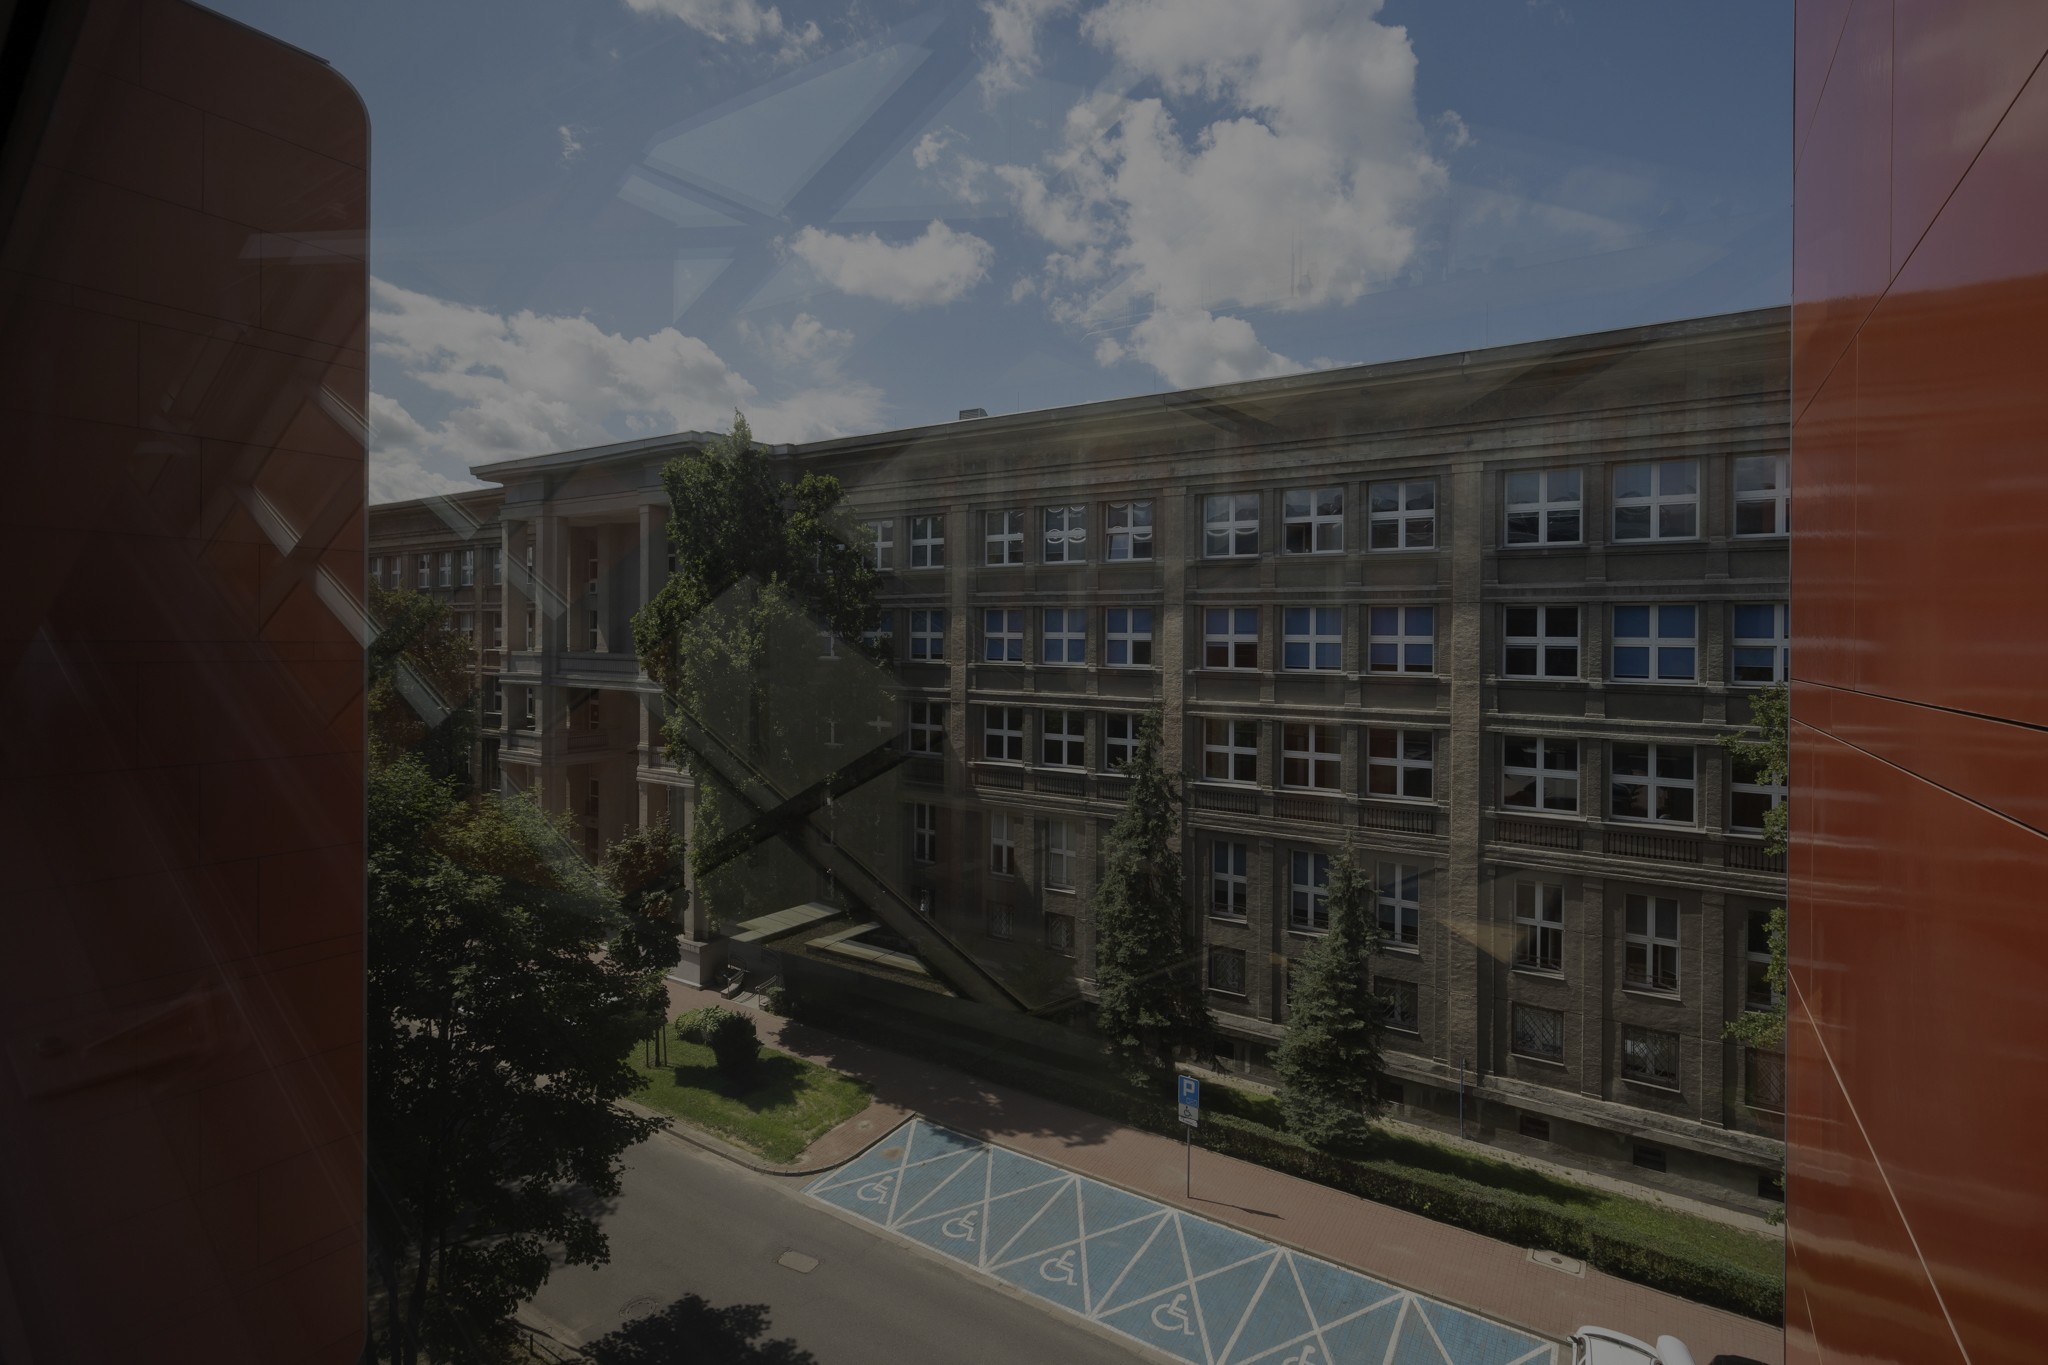
\includegraphics[height = \paperheight]{rozdziały/images/mimuw.jpg}
    }
}

% --- Nagłówki sekcji
\definecolor{headingColor}{HTML}{8bc95c}

\titleformat{\chapter}[hang]{\sffamily}{
    \begin{tcolorbox}[
        extrude top by = 5cm,
        enlarge bottom finally by = -3.2mm,
        frame hidden,
        colback = headingColor,
        coltext = white,
        hbox,
        sharp corners = north,
        rounded corners = south,
        arc = 5mm
    ]
        {\fontsize{50}{60}\selectfont \thechapter}
    \end{tcolorbox}
}{2.5em}{\Huge\bfseries}

\titleformat{\section}{\sffamily\Large\bfseries}{
    \begin{tcolorbox}[
        enlarge bottom finally by = -3.2mm,
        grow to left by = 3.1cm,
        frame hidden,
        colback = headingColor,
        coltext = white,
        width = 3.5cm,
        halign = right,
        arc = 5mm
    ]
        {\thesection.}
    \end{tcolorbox}
}{1em}{}

\titleformat{\subsection}
{\sffamily\large\bfseries}{\textcolor{headingColor} {\LARGE $\blacksquare$}}{1em}{}

% --- Stopka
\renewpagestyle{plain}{
    \setfoot[
        \begin{tcolorbox}[
            enlarge bottom finally by = -1mm,
            grow to left by = 3.1cm,
            frame empty,
            colback = headingColor,
            coltext = white,
            width = 3.5cm,
            height = 4mm,
            size = tight,
            rightupper = 2mm,
            halign = right,
            valign = center,
            sharp corners = all
        ]{\sffamily\footnotesize\bfseries\thepage}
        \end{tcolorbox}
        \ifthechapter{\hspace{0.5cm} \sffamily\footnotesize\thechapter. \chaptertitle}{}
    ][][] % parzyste strony
    {}{}{
        \ifthesection{\sffamily\footnotesize\thesection. \sectiontitle \hspace{0.5cm}}{}
        \begin{tcolorbox}[
            enlarge bottom finally by = -1mm,
            grow to right by = 3.1cm,
            frame empty,
            colback = headingColor,
            coltext = white,
            width = 3.5cm,
            height = 4mm,
            size = tight,
            leftupper = 2mm,
            valign = center,
            sharp corners = all
        ]{\sffamily\footnotesize\bfseries\thepage}
        \end{tcolorbox}
    }} % nieparzyste strony
\pagestyle{plain}

% --- Kolorowanie linków
\hypersetup{
    colorlinks = true,
    linkcolor = headingColor,
    filecolor = headingColor,
    urlcolor = headingColor
}
\urlstyle{same}

% --- Spis treści
\renewcommand{\cfttoctitlefont}{\sffamily\Huge\bfseries}
\renewcommand{\cftchapfont}{\sffamily\large\bfseries}
\renewcommand{\cftchapafterpnum}{\vspace{4pt}}
\renewcommand{\cftchapaftersnum}{.}
\renewcommand{\cftsecaftersnum}{.}

% --- Ramki
\definecolor{exampleColor}{HTML}{f89b0f}
\definecolor{exampleSubtitleColor}{HTML}{ffdba0}
\definecolor{examColor}{HTML}{40bfdf}
\definecolor{examBackgroundColor}{HTML}{f3fbfd}
\definecolor{problemsColor}{HTML}{f89b0f}
\definecolor{problemsBackgroundColor}{HTML}{fefddf}
\definecolor{solutionsColor}{HTML}{66c430}
\definecolor{solutionsBackgroundColor}{HTML}{f0f9e6}
\definecolor{editorsNoteColor}{HTML}{c53119}
\definecolor{editorsNoteBackgroundColor}{HTML}{ffe9e6}

\tcbset{
    enhanced,
    parbox = false,
    colback = white,
    colbacktitle = white,
    coltitle = black,
    fonttitle = \sffamily\bfseries,
    attach boxed title to top left = {
        yshift = -\tcboxedtitleheight/2,
        yshifttext = -\tcboxedtitleheight/2
    },
    boxed title style = {
        interior code = {
            \path [tcb fill interior] (frame.north west) -- (frame.north east) -- ([xshift = 2mm]frame.east) -- (frame.south east) -- (frame.south west) -- cycle;
            \draw [color = tcbcolframe, line width = 0.2mm] (frame.north west) -- (frame.north east) -- ([xshift = 2mm]frame.east) -- (frame.south east) -- (frame.south west);
            \draw[color = tcbcolframe, line width = 1mm] ([xshift = 0.5mm]frame.south west) -- ([xshift = 0.5mm]frame.north west);
        }
    },
    arc = 2mm,
    sharp corners = west,
    boxrule = 0.2mm,
    leftrule = 1mm,
    enlarge top by = 1mm,
    enlarge bottom by = 1mm
}

\newtcolorbox[
    auto counter,
    number within = section,
    number freestyle = {\noexpand\arabic{\tcbcounter}.},
]{example}{
    breakable,
    title = Przykład \thetcbcounter,
    colframe = exampleColor,
    subtitle style = {
        hbox,
        frame empty,
        colback = exampleSubtitleColor,
        fontupper = \rmfamily\bfseries
    },
    oversize
}

\newtcolorbox{exam}{
    breakable,
    title = To było na egzaminie,
    coltitle = white,
    colbacktitle = examColor,
    colframe = examColor,
    colback = examBackgroundColor,
    oversize
}

\newtcolorbox{problemsf}{
    breakable,
    sharp corners = all,
    spread sidewards,
    colbacktitle = problemsColor,
    coltitle = white,
    colframe = problemsColor,
    colback = problemsBackgroundColor,
    title = \hspace{1.8cm} Zestaw zadań,
    left = 2.4cm,
    right = 2.4cm,
    leftrule = 0pt,
    rightrule = 0pt
}

\newtcolorbox{solutionsf}{
    breakable,
    sharp corners = all,
    spread sidewards,
    colbacktitle = solutionsColor,
    coltitle = white,
    colframe = solutionsColor,
    colback = solutionsBackgroundColor,
    title = \hspace{1.8cm} Rozwiązania,
    left = 2.4cm,
    right = 2.4cm,
    leftrule = 0pt,
    rightrule = 0pt
}

\newtcolorbox{editorsnote}{
    breakable,
    title = Przypis redakcji,
    coltitle = white,
    colbacktitle = editorsNoteColor,
    colframe = editorsNoteColor,
    colback = editorsNoteBackgroundColor,
    oversize
}